\documentclass[letterpaper]{article}
\usepackage{aaai}
\usepackage{amsmath}
\usepackage{pgfplots}
\usepackage{caption}
\usepackage{apacite}
\usepackage{subfig}

\RequirePackage{booktabs}
\setlength{\pdfpagewidth}{8.5in} 
\setlength{\pdfpageheight}{11in}


\setcounter{secnumdepth}{0}
\pgfplotsset{compat=1.12}

\title{Playing Card recognition using Convolutional Neural Network}
\author{Gregory Poisson, Bradley Winters \and Joshua O'Dell \\ Colorado State University \\ Fort Collins, CO 80523 }
\begin{document}
\maketitle

\section{Abstract}

One of the most important technological advancements in the last few years has been the availability of image recognition algorithms and libraries.  This paper will explore an image recognition system which utilizes a convolutional neural networks to recognize images of playing cards. We discuss the use of such a neural network, and the issues that arose as we began to implement it.  We will touch on the problems that we solved, as well as the problems for which a solution was not found.  Finally, we will give a summary of our experience, discuss the current efficacy of the technology, and remark upon different applications of our results.

\section{Introduction}

In this paper we aim to implement a playing card image recognition system.  This system could have numerous uses, allowing for automated players, or assistants, to identify and potentially interact with cards on the table. In this way, computerized opponents might be made which could play more than simple graphical card games, but also physical ones using paper cards.
The image recognition industry has progressed quickly, there are several tools available for doing image recognition.  Our paper will focus on a neural network with convolution layers.

\section{Methods}
To convey exactly how this system is designed, we present a general description of the implementation we used.

\subsection{Homemade Neural Network}
We started the study with a handwritten neural network class.  It was a simple class written in Python with the ability to create convolutional layers.  The results of using this class were unsatasfactory, however.  The training time took days to train on anything with more then a single convolutional layer.  We therefore decided to look at other commercial and open source libraries which had been developed by companies with far more resources then our team.

\subsection{TensorFlow}
One of the libraries that first came up was Google's TensorFlow library \cite{tensorflow}.  This library is freely available and has the ability to produce simple, easily understand assets.  We settled on using this library.
Tensorflow features a pretrained model named inception V3.  This model has been trained with 1.2 million images representing 1000 classes.  Fully training an image classifier on thousands of images would have taken weeks or months.  We opted instead to retrain the final 2 layers of the inception V3 model for playing cards.  These layers consist of a bottleneck or autoencoder layer and a final classifcation layer.  In essence, the classifier is identifying playing cards with features learned from other images. 

\subsection{Training Data}
To train our neural network, we needed images of all 52 playing cards in a standard deck of playing cards.  We started by manually taking approximately 20 photographs of each playing card in a deck, then placing them in separate folders with a naming convention that TensorFlow could use.  We then copied and manipulated these images, skewing, rotating, and cropping them using an automated script. Our dataset in total contained approximately 6,500 images.

\subsection{Initial tests}
We began by training our neural network on approximately 1,000 images, just to see how accurate our initial predictions would be. As shown in Figure~\ref{fig:initial_results_1}, results varied for cards with complex backgrounds, but the model was confident about cards with little to no background image data. 
\begin{figure}
  \centering
  \subfloat[47\% confidence]{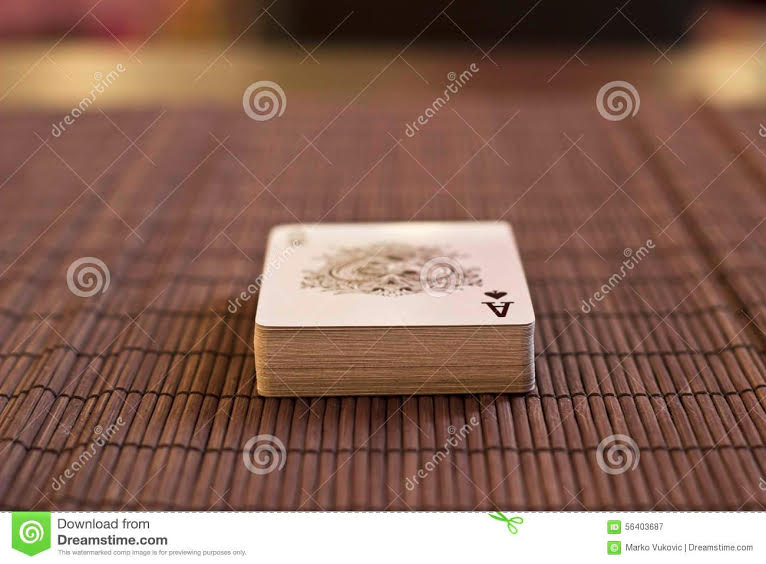
\includegraphics[width=0.2\textwidth]{initialresults/ace_spades_1.jpg}}
  \subfloat[73\% confidence]{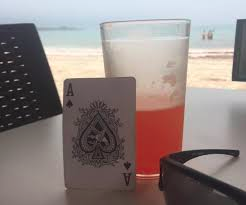
\includegraphics[width=0.2\textwidth]{initialresults/ace_spades_2.png}}

  \subfloat[45\% confidence]{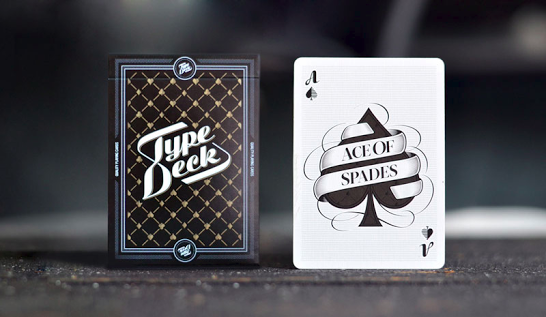
\includegraphics[width=0.2\textwidth]{initialresults/ace_spades_3.png}}
  \subfloat[91\% confidence]{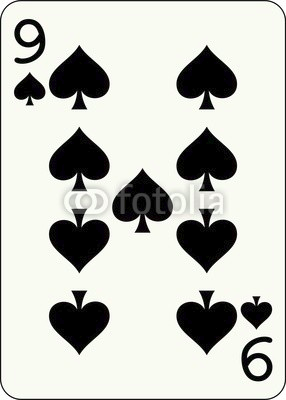
\includegraphics[width=0.2\textwidth]{initialresults/ace_spades_4.png}}
  \caption{\label{fig:initial_results_1} Correctly classified images with class probabilities; initial classifier}
\end{figure}

% card subset =
% 4 of clubs
% 4 of spades
% 4 of hearts
% 4 of spades
% 9 of spades
% A of spades
% A of hearts

We hypothesized that the network needed more training data, and more training steps. 1,000 images was not a large dataset, and the fact that we were seeing results already was promising.

\subsection{Refining the Training}
With the success of the initial tests we began to train the network in ernest. We supplemented the photographs in our dataset with card images obtained from Google. We added 8 such images for each card (class), then trained the network on a set of 1,800 training images using 1,600 training steps.  This training took several hours, but the results were even better.  The network was now able to more accurately classify images with various backgrounds. Figure~\ref{fig:refining_results_1} shows some examples of the images with cards that were now correctly classified, as well as examples of the training images without backgrounds, which greatly refined our model.

\begin{figure}
  \centering
  \subfloat[18\% confidence]{\label{fig:refining_results_11} 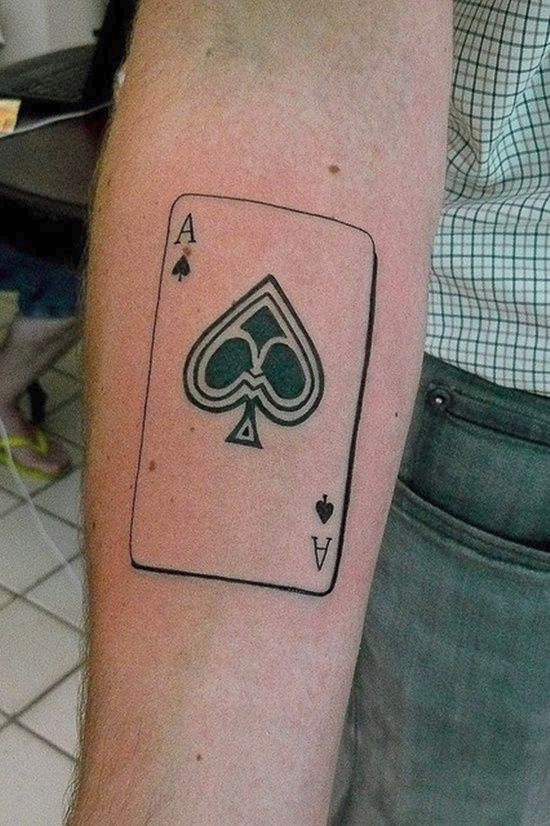
\includegraphics[width=0.2\textwidth]{refining/unnamed.png}}
  \subfloat[79\% confidence]{\label{fig:refining_results_12} 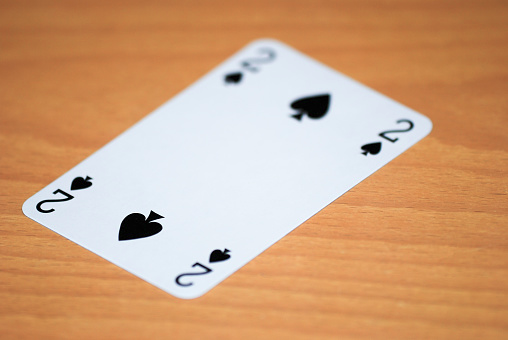
\includegraphics[width=0.2\textwidth]{refining/2_spades.png}}

  \subfloat[36\% confidence]{\label{fig:refining_results_13} 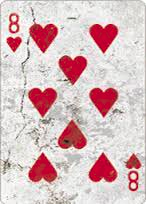
\includegraphics[width=0.2\textwidth]{refining/8_hearts.png}}
  \subfloat[69\% confidence]{\label{fig:refining_results_14} 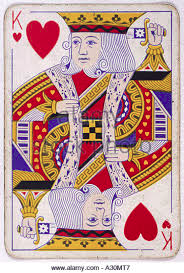
\includegraphics[width=0.2\textwidth]{refining/k_hearts.png}}
  \caption{\label{fig:refining_results_1}Figure~\ref{fig:refining_results_11}, \ref{fig:refining_results_12} images with complex backgrounds correctly classified. Figure~\ref{fig:refining_results_13}, \ref{fig:refining_results_14} images with no backgrounds, used for training}
\end{figure}



\subsection{OpenCV}
One of our initial goals was to be able to recognize as many situations as we could, including cards that were not oriented in a way that our network was trained to handle.  We also wanted to be able to recognize multiple cards within the same image.  What we found was that our network was able to recognize cards oriented horizontally or vertically, it had a hard time with rotated cards, skewed cards, and was terrible with multiple cards on the same image.

Our solution was to pre process the images.  First the cards are isolated in the image, and then they are transformed to be flat rectangular images, which are then classified through the trained network.  Using code inspired from \cite{openCV1} and \cite{openCV2} we leveraged the OpenCV library to locate and transform the card into a clean, flat piece of data prior to classification.  Figure~\ref{fig:opencv_1} shows an example of pre processing and pulling out the playing card portion of the image.

\begin{figure}
  \centering
  \subfloat[OpenCV extracting the 8 of Spades from an image with multiple cards]{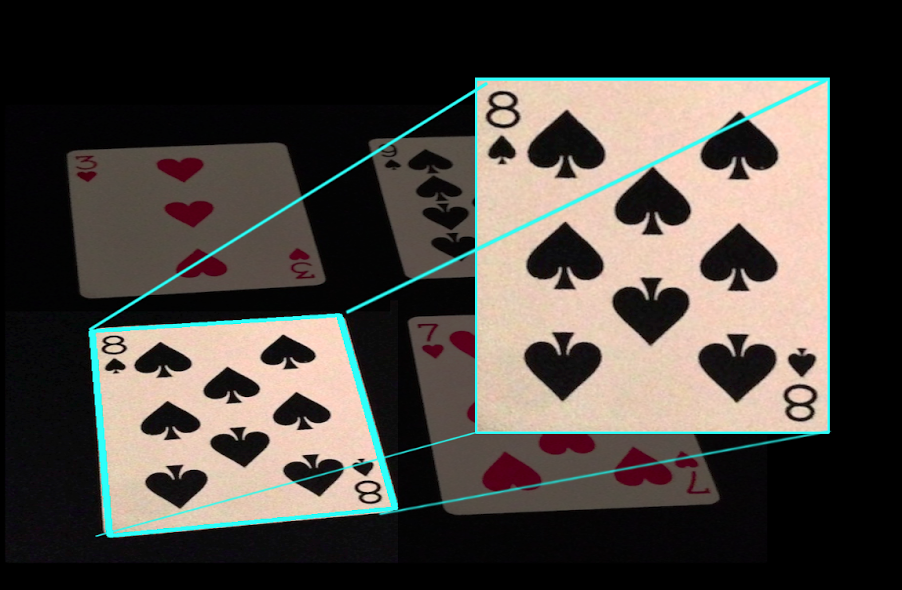
\includegraphics[width=0.4\textwidth]{opencv/demo.png}}

  \subfloat[Pre processed Ace of Spades]{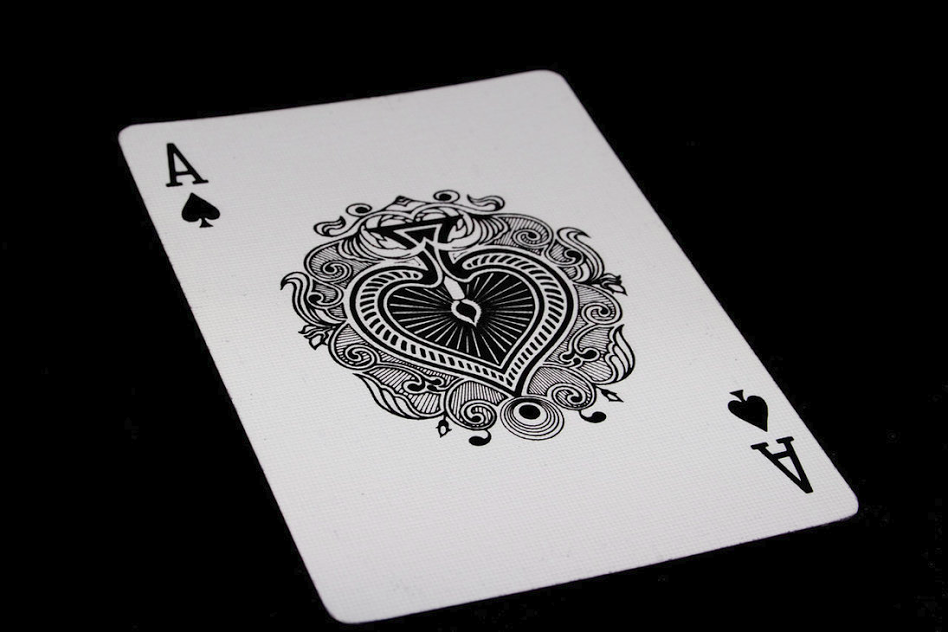
\includegraphics[width=0.2\textwidth]{opencv/ace_spades_1.png}}
  \subfloat[Post processed Ace of Spades]{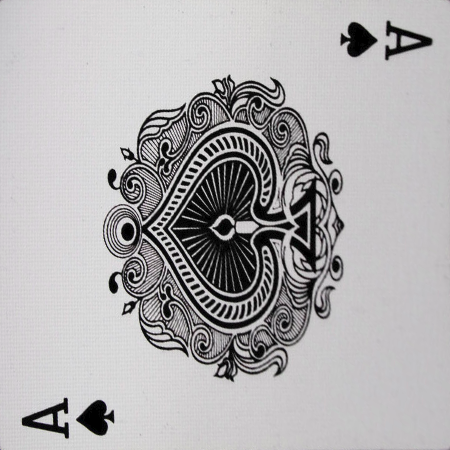
\includegraphics[width=0.2\textwidth]{opencv/ace_spades_2.png}}
  \caption{\label{fig:opencv_1} OpenCV pre-processing on images}
\end{figure}


\section{Results and Discussion}
Upon implementing OpenCV and expanding the training dataset to include images which did not contain backgrounds, we trained a classifier over 32,000 epochs. This training was performed on a CPU and ran overnight. 
The classifier we trained exhibited a 90\% accuracy on test data. Figure~\ref{fig:confus} shows the confusion matrix for this model with respect to all 52 classes.  Examining the confusion matrix we were hard pressed to find a pattern of misclassification.  While the system did achieve a 90\% success rate, it could certainly perform better.  However at this point we were hard pressed to find a misclassification that could easily be trained out.

We also experimented with classifying images which contained more than one card. Figure~\ref{fig:opencv_1}(a) gives an example of this. The process which worked best was to convert the image to black and white, based on a pixel intensity threshold, and to then isolate and rotate the cards before classifying them one at a time.
\begin{figure}[!tbp]
  \centering
  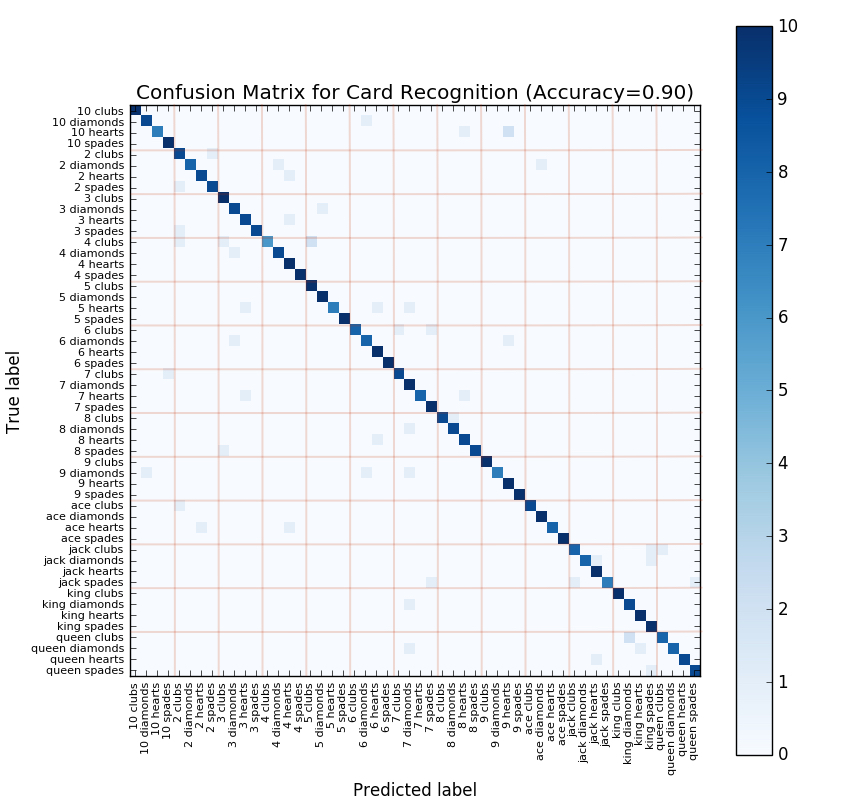
\includegraphics[width=0.6\textwidth]{results/confusion2.jpg}
  \caption{\label{fig:confus}Confusion matrix for classifier after 32,000 training epochs with a test set size of 520 cards (10 per card)}
\end{figure}

We found that even at 32,000 epochs our model was still increasing its accuracy.  However given time limitations of this project, and a need to create accurate performance measurements we stopped the training at this point.

\section{Conclusions}
The learning architecture of the neural network in TensorFlow began to show a capacity for classifying playing cards almost immediately. However, by including enhancements such as training data without extraneous information, and the pre processing capability of OpenCV, we found we were able to substantially increase the classification power of our model. With enough training, we found that our dataset and model structure allowed us to achieve a maximum out of sample accuracy of 90\%. 

Next steps to continue this research project would be to further examine the cards that were misclassified, to try and discern a patter, and possibly train those errors out of the model by selecting additional training sets.  It would also be possible to examine other libraries, and compare results.  However, the equations and code used for convolution layers within a neural network are common, and aside from performance differences, we would not anticipate the results to be much better or worse.

There is no current state of the art in card classification, but image classification itself has become a booming field.  We found that a single solution of applying a neural network was not on its own sufficient.  We needed to add pre processing and other technologies to the solution.  Our accuracy is not quite production ready, but clearly demonstrates the potential of this method as a proof-of-concept that could be implemented in an interface to allow computers and humans to play various card games.


\nocite{*}
\bibliographystyle{apacite}
\bibliography{references}

\section{Work Breakdown}

\subsection{Gregory Poisson}

Training / validation data creation

TensorFlow testing

report: Methods details, conclusion

\subsection{Bradley Winters}

Neural Network Class testing

TensorFlow model creation, output consolidation

OpenCV calculation initial setup

report: implementation details

\subsection{Joshua O'Dell}

Home built Neural network

TensorFlow testing

report: first draft of all sections, latex structure, final proofing.

\end{document}

